\section{Performance Characterization under the SFJ limit}
\label{sec:tolerant}

In this section, we characterize the performance of the $\t$-class and
the $\i$-class under the SFJ limit.

Recall that in our system, both classes are scheduled in a
\emph{dynamic} manner, with the $\i$-sub-policy being selected based
on current $\t$-occupancy, and the $\t$-queue in turn being served (in
a work conserving fashion) using the unused service process of the
$\i$-sub-policy. Thus, the two classes experience random, time
varying, state-dependent, and also \emph{inter-dependent} service
processes. This makes a precise performance evaluation intractable;
indeed, no closed form characterization of the performance of the
tolerant class is possible even in the simplified setting where the
eager class is scheduled by a policy that is oblivious to the tolerant
state; see \cite{Mahabhashyam05,ANOR}. In this section, we show that
under the (partially fluid) SFJ scaling, tractable performance
characterizations are possible.


To provide intuition for the form of our results, recall that the
timescale separation resulting from the SFJ scaling results in the
tolerant queue obtaining, in the limit, service at a `steady' rate of
$\nu_{j} := 1 - \rho_\epsilon \left(1 - P_{B_j}\right)$ when there are
$j$ tolerant jobs in the system. Here, $P_{B_j}$ is the standalone, or
$\t$-static blocking probability associated with sub-policy~$j.$ One
might then anticipate that the limiting performance of the tolerant
class is described in terms of a system with a state-dependent service
rate, i.e., where the service rate is a (deterministic) function of the
queue occupancy. We prove that this is indeed the case. Before we
state our main results, we first describe this limit system, which we
refer to as a state-dependent service rate M/M/1 (SDSR-M/M/1) queue.


\subsection{State-dependent service rate M/M/1 queue}

An SDSR-M/M/1 queue sees the same arrival process as an M/M/1 queue:
job arrivals are according to a Poisson process (of rate
$\lambda$). Further the job sizes are independent and exponentially
distributed with mean $1/\mu$. However, unlike the standard M/M/1
queue, the SDSR-M/M/1 queue has a state dependent service rate
(a.k.a. server speed). Specifically, the server operates with service
rate $\nu_j$ if the number of jobs in the queue (including the job in
service) equals $j.$ Thus, the SDSR-M/M/1 queue is parametrized by
$(\lambda, \mu, \bm{\nu})$, where $\bm{\nu} = \{\nu_j\}_{j \geq 0}$ is
the vector of service rates.


The number of jobs in the SDSR-M/M/1 queue evolves as a continuous
time Markov process with birth-death structure (see Figure
\ref{Fig_SDSR-system}). 
\begin{figure}
	\begin{center}
		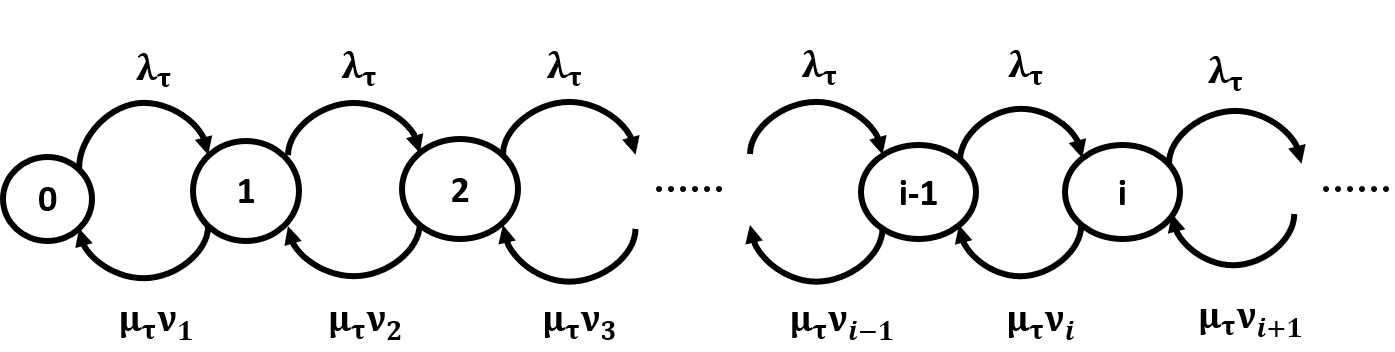
\includegraphics[width= .9 \textwidth]{SDSR-system.PNG}
		\caption{SDSR-M/M/1 queue with parameter $(\lambda_\t, \mu_\t, \bm{\nu} = \{\nu_1, \nu_2, \nu_3, \cdots\}).$}
		\label{Fig_SDSR-system}
	\end{center}
\end{figure}
Moreover, Assumption~{\bf B.}4 ensures that this Markov process is
positive recurrent. Thus, its steady state distribution can be
obtained by elementary techniques. In particular, the stationary
distribution ${\bm \pi} := \{\pi_{i} \}_{i = 0}^{\infty}$, is given by
(see \cite{Gallager2012}):
\begin{eqnarray}
\label{Eqn_SDSR_SD}
\pi_{i}   &=&   \frac{  \indicator{i=0} + \indicator{i \ge 1}  \prod_{\ell=1}^i \rho_{\ell} }{1 + \sum_{k \ge 1}    \prod_{\ell=1}^k \rho_{\ell} } \  
\mbox{,}  \  \rho_{\ell} :=  \frac{\lambda_\t}{\mu_\t \nu_{\ell}}.
\end{eqnarray}


\subsection{Main results}

Recall that the scheduler is specified by a sequence of eager
sub-policies one for each tolerant occupancy; $P_{B_j}$ being the
$\t$-static probability of the eager sub-policy used under tolerant
occupancy $j$. The performance of the tolerant class under the SJF
limit, and under any scheduler, is characterized as follows. The
steady state occupancy of the tolerant queue converges, in
distribution, and also in expectation, to the corresponding quantities
of an SDSR-M/M/1 system parameterized by
$(\lambda_\t, \mu_\t, \bm{\nu}).$

\begin{thm} {\bf{[Stationary distribution of $\t$-occupancy}]}
\label{Thm_Lim_SD_Conv}
Assume $\bm{A}$.1-4 and $\bm{B}$.1-4. Under the SFJ limit, the steady
state number $\t$-occupancy converges in distribution to
the steady state occupancy in an SDSR-M/M/1
$(\lambda_\tau, \mu_\tau, (\nu_1, \nu_2, \cdots ))$ queue, with
  $$
  \hspace{10mm}
  \nu_j :=    ( 1-  \rho_\epsilon (1-{P_B}_j) ) ,  \mbox{ for }  j \geq 0.
  $$
  That is,
  $$
  {\pi}_i^\mue \stackrel{\mue \to \infty}{\longrightarrow} {\pi}_i \ \mbox{for all} \  i \geq 0, 
  $$ where ${\pi}_i$ is given by \eqref{Eqn_SDSR_SD}.
\end{thm}


\begin{thm} {\bf [Stationary expected $\t$-occupancy]}
\label{Thm_tau}
Assume $\bm{A}$.1-4 and $\bm{B}$.1-4. Under the SFJ limit, the
stationary expected number of $\t$-customers converges to that of the
limit system described in Theorem~\ref{Thm_Lim_SD_Conv}. That is,
\begin{eqnarray*}
\label{Eqn_SDSR_Expected_Number}
   E^\mue[N] \stackrel{\mue \to \infty}{\longrightarrow}  \sum_{i=1}^\infty i \pi_{i},
\end{eqnarray*}
where ${\pi}_i$ is given by \eqref{Eqn_SDSR_SD}.
\end{thm}

Given that ${\bm \pi} := \{\pi_{i} \}_{i = 0}^{\infty}$ is the
stationary distribution of a simple birth-death CTMC,
Theorems~\ref{Thm_Lim_SD_Conv} and~\ref{Thm_tau} provide closed form
characterizations of the limiting performance of the tolerant class
under the SFJ scaling. It is important to note that while the
statements of Theorems~\ref{Thm_Lim_SD_Conv} and~\ref{Thm_tau} might
seem intuitive, their proofs are rather involved. In particular, they
rely crucially on a \emph{uniformity} in the convergence of the
service process seen by the tolerant queue under the SFJ limit,
\emph{across $\i$-sub-policies}; see
Subsection~\ref{sec:tol_perf_proofs}.


Next, we describe the performance of the eager class under the SFJ
limit, which is captured by its blocking probability, i.e., the long
fraction of eager customers blocked. Formally, the blocking
probability is defined as follows. Let $N_B^\mue (t)$ denote the total
number of eager customers that are blocked (i.e., returned without
service), before time $t$ and $N_A^\mue (t)$ be the total number of
eager customers arrived in the same time interval, for the system at
scale $\mu_\i.$
% and under any given dynamic policy.
Then the blocking probability of the eager class is defined as the
long run fraction of customers blocked, i.e.,
\begin{equation}
  \label{eq:PB-def}
P_B^\mue := \lim\limits_{t \to \infty } \frac{N_B^\mue (t)}{N_A^\mue (t)}.
\end{equation}
Note that eager jobs are blocked by different sub-policies, which
operate dynamically based on the occupancy of the tolerant
queue. Thus, it is not a priori even clear that the limit in
\eqref{eq:PB-def} exists almost surely. That it does, and that the
eager blocking probability converges under the SFJ limit to a convex
combination of the $\t$-static blocking probabilities $\{ P_{B_j}\},$
weighted by the (limiting) long run fractions of time the $\t$-system
spends in each state, is established by the following theorem.

\begin{thm} \textbf{[Blocking probability of eager class]} 
\label{Thm_PB}
Assume {\bf A}.1-4, {\bf B}.1-4. Then the steady state blocking
probability of $\epsilon$-jobs in SFJ limit is given by:
{\small
  \begin{align*}
    \hspace{25mm} 
    \hspace{5mm}
    P_B^{\mu_\epsilon} \ \ \stackrel{\mu_\epsilon \to
  \infty}{\longrightarrow} \ \
\sum_{j=1}^{\infty } {P_B}_j {\pi}_j =: P_B^{\infty},
    \hspace{25mm} 
  \end{align*}}
where ${\pi}_i$ is given by \eqref{Eqn_SDSR_SD}.
\end{thm}

A key takeaway from Theorems~\ref{Thm_Lim_SD_Conv}--\ref{Thm_PB} is
that the performance of both classes under the SFJ limit can be
characterized in terms of the $\t$-static blocking probabilities
$\{ P_{B_j} \}_{j \geq 0}$. The probabilities
$\{ P_{B_j} \}_{j \geq 0}$ themselves are typically easy to compute,
since they involve the analysis of a single-class (stationary) loss
system. Thus, by virtue of
Theorems~\ref{Thm_Lim_SD_Conv}--\ref{Thm_PB}, we have the following
conservation law.

\noindent {\bf Dynamic Pseudo Conservation}: Under the SFJ limit, the
performance of \emph{both} classes depends only on the $\t$-static
blocking probabilities $\{ P_{B_j} \}_{j \geq 0}$ and not the
specifics of the $\i$-sub-policies that produced these blocking
probabilities.

\revision{Finally, since Assumption {\bf A}.1 may seem unreasonable,
  we show below that the conclusions of
  Theorems~\ref{Thm_Lim_SD_Conv}-\ref{Thm_PB} hold even without this
  assumption, if eager job sizes are taken to be exponentially
  distributed.
  % hence we provide another result without that
  % assumption.  We instead assume that the $\i$-service times are also
  % exponentially distributed.  We show below that all the previous
  % results are valid for this case also (proof is in Appendix).
  \begin{thm}
    \label{Thm_withou_A1}
    Assume {\bf A}.2-4 and {\bf B}.1-4. Also assume that the
    $\i$-service times are exponentially distributed. 
The
    conclusions of Theorems~\ref{Thm_Lim_SD_Conv}-\ref{Thm_PB} hold, once   the
    transitions between eager sub-policies are handled  as described in
    Section~\ref{sec:example_models} (i.e., following an
    arrival/departure in the tolerant queue, the new eager sub-policy
    dictates the scheduling of the eager queue from then on).
  \end{thm}
  Theorem~\ref{Thm_withou_A1} shows that Assumption {\bf A}.1 is
  benign, i.e., it does not affect the performance of either class
  under the SFJ limit. As expected, the proof of
  Theorem~\ref{Thm_withou_A1} is considerably more involved as
  compared to the proofs of
  Theorems~\ref{Thm_Lim_SD_Conv}-\ref{Thm_PB}. Specifically,
  Assumption {\bf A}.1 allows the evolution of the $\t$ queue (across
  arrival/departure epochs) to be described by a one-dimensional
  birth-death Markov chain (see
  Section~\ref{sec:tol_perf_proofs}). This is no longer possible in
  the absence of Assumption {\bf A}.1; the system evolution has to be
  captured via a certain two-dimensional Markov chain, whose long-run
  time averages must be shown to match those corresponding to the
  former birth-death chain as $\mue \ra \infty$ (see
  Appendix~\ref{app:withoutA1}).
%  We then show that this Markov chain in positive recurrent for large
%  enough $\mue,$ and that the transition probabilities converge
%  uniformly as $\mue \ra \infty.$
}



We note that while our performance characterization is derived under
the SFJ limit, we show in Section~\ref{sec:pareto} that they provide
accurate approximations of the performance experienced in the
pre-limit. The remainder of this section is devoted to highlighting
the main steps in the proofs of Theorems~\ref{Thm_Lim_SD_Conv}
and~\ref{Thm_tau}. Most details are relegated to
Appendix~\ref{Appendix_tolerant}. The proof of Theorem~\ref{Thm_PB} is
presented in Appendix~\ref{Appendix_eager}. \revision{The proof of
  Theorem~\ref{Thm_withou_A1} can be found in
  Appendix~\ref{app:withoutA1}.}

\subsection{Analysing tolerant performance under the SFJ limit}
\label{sec:tol_perf_proofs}

\begin{figure}
\begin{center}
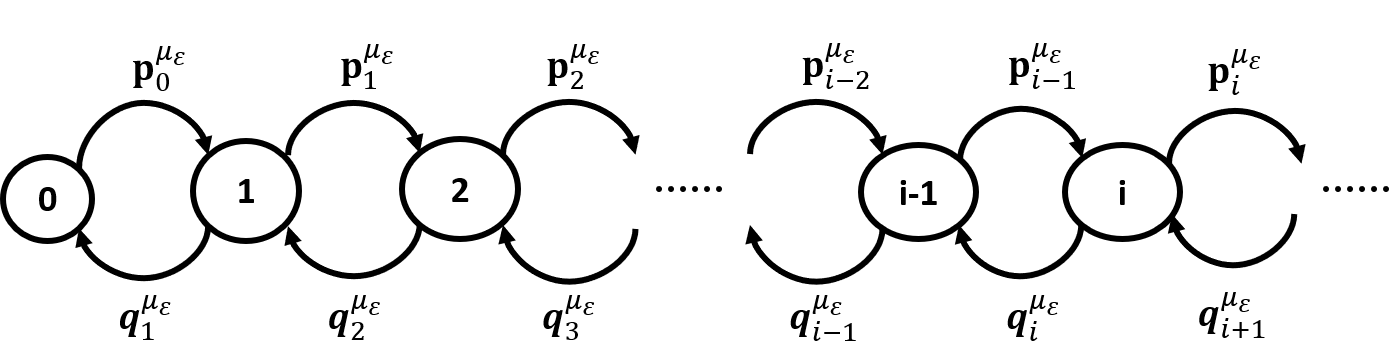
\includegraphics[width= .9 \textwidth]{StateTransitionPre-Limit2.PNG}
\caption{State Transition $\tau$-queue corresponding to eager service
  rate $\mue$.}
\label{Fig_StateTrans_PreLimit}
\end{center}
\end{figure}

\revision{We now sketch the main steps in the proofs of
  Theorems~\ref{Thm_Lim_SD_Conv} and~\ref{Thm_tau} (i.e., under
  Assumption {\bf A}.1).} We characterize the $\t$-performance by
first analysing the $\t$-queue at its arrival/departure epochs. Let
$X_n$ denote the occupancy of the $\t$-queue immediately following the
$n$th arrival/departure. Under Assumption~{\bf A}.1 (dropping of
existing $\i$-customers at $\t$-transitions) and because of
exponentially distributed tolerant job sizes, $\{X_n\}$ is a
discrete-time Markov chain with birth-death (BD) structure; see
Figure~\ref{Fig_StateTrans_PreLimit}. Let $p_j^\mue$ and $q_j^\mue$,
respectively, denote the forward and backward transition probabilities
of this (pre-limit) tolerant BD chain, when there are $j$ tolerant
customers in the system.  Let $A_\tau$ and $B_\tau$ represent, a
generic inter-arrival time associated with the tolerant queue, and a
generic tolerant job size, respectively. Also,
recall~$\Upsilon_j^{\mu_\epsilon}(B_\t)$ denotes the time required to
finish $B_\tau$ amount of work using the service
process~$\Omega^{\mu_\epsilon}_{j}(\cdot)$ (see
Section~\ref{sec:background}), then we have:
\begin{equation*}
  \label{eq:q_j-def}
q^{\mue}_j = 1 - p^{\mue}_j:= \prob{A_{\t} > \Upsilon^{\mu_\epsilon}_j(B_\t)}.
\end{equation*}
Observe by {\bf A}.1 that the job completion times, distributed as
$\Upsilon_j^{\mu_\epsilon}(B_{\t }) $, are i.i.d.  across all those
customers that were served when the tolerant occupancy
equals~$j$. Moreover, if such a tolerant service is interrupted by a
$\t$-arrival, the remaining completion time is distributed as
$\Upsilon_{j+1}^{\mu_\epsilon}(B_{\t} ),$ thanks to the memoryless
property of tolerant job sizes and~{\bf A}.1.

Our first step is to prove that the above transition probabilities
converge to the transition probabilities associated with the embedded
BD chain corresponding to the
$(\lambda_\tau, \mu_\tau, (\nu_1, \nu_2, \cdots ))$ SDSR-M/M/1
system. Moreover, we show that \emph{the above convergence takes place
  uniformly over sub-policies~$j.$} Before stating this result, we
recall the definition of uniform convergence (which we denote by
$u.f.$):
%

\textbf{Definition:} $\left[\textbf{Uniform
    $(u.f.)$ convergence }\right]$ A parameterized family of sequences
$\{x_{j}^{\mue}\}_{j \geq 0}$ is said to be uniformly convergent to
the limit $\{x_j\}_{j \geq 0}$ as $\mue \ra \infty$ if, for every
$\epsilon >0$ there exists $\bar{\mu}$, such that
$$
\left| x_{j}^{\mue} - x_j \right| < \epsilon \ \ \mbox{for all} \ \
\mue > \bar{\mu} \mbox{ and for all } j \geq 0.
$$ 
% 
\begin{lemma}
	\label{Lem_TP_Convergence}
	$\left[\textbf{Uniform convergence of transition
            probabilities}\right]$ i) If $p_j^\mue$ denotes the
        probability of a $\t$-arrival before a $\t$-departure in the
        (pre-limit) system when the number of tolerant customers in
        the system equals $j$, then
	\begin{eqnarray}
	\label{eq:q_conv}
	p_j^\mue \stackrel{\mue \to \infty}{\rightarrow} p_j^{\infty} := \frac{\lambda_\t}{\lambda_\tau + \nu_j \mu_\tau} \ \mbox{and } \ q_j^\mue := 1 - p_j^\mue   \stackrel{\mue \to \infty}{\rightarrow} q_j^{\infty}:= \frac{\nu_j \mu_\t}{\lambda_\tau + \nu_j \mu_\tau} . 
	\end{eqnarray}
	\label{lemma:uniform}
	ii) The convergence in \eqref{eq:q_conv} occurs u.f. over the
        sub-policies $j$.  Precisely, for every $\epsilon > 0$ there
        exists $\bar{\mu} > 0$, such that for all
        $\mu_\epsilon \geq \bar{\mu}$ and for all $j \geq 0,$ we have:
	\begin{eqnarray}
	\bigg| q_j^{\mu_\epsilon} - \frac{\nu_j \mu_\tau}{\lambda_\tau + \nu_j \mu_\tau}  \bigg| < \epsilon.
	\end{eqnarray} 
	%$ \in \g.$
\end{lemma}
The proof of Lemma~\ref{Lem_TP_Convergence} is provided in
Appendix~\ref{sec:lemma:uniform}.


The next step is to show that the embedded BD chain characterizing the
evolution of the occupancy of tolerant queue is positive recurrent for
large enough $\mue.$
%
\begin{lemma}
  \label{lemma:TauStability}
  There exists $\bar{\mu} > 0$ such that for $\mue > \bar{\mu},$ the
  (embedded) Markov chain $\{X_n\}$ is positive recurrent.
\end{lemma}
The proof of Lemma~\ref{lemma:TauStability} is provided in
Appendix~\ref{sec:lemma:TauStability}. Lemma~\ref{lemma:TauStability}
also implies that for large enough $\mue,$ the $\tau$-queue is stable
and has a well defined stationary behaviour.\footnote{The occupancy of
  the tolerant queue evolves as a semi-Markov process in continuous
  time. The regularity of this process (i.e., each state is visited
  only finitely often in any finite interval of time with
  probability~1) follows by noting that the number of state
  transitions is lower bounded by those in a standard M/M/1 queue with
  arrival rate $\lambda_\t$ and service rate $\mu_\t$. The positive
  recurrence of this process follows from Theorem~5.9 in
  \cite{Gallager2012}, noting that mean residence time in any state is
  uniformly upper bounded by $1/\lambda_\t.$} The stationary
distribution for $\mue > \bar{\mu}$ can be calculated using standard
techniques and is given by (see, for example,~\cite{Hoel}),
\begin{eqnarray}
\label{Eqn_SD_pre-limit}
\tilde{\pi}_i^\mue = \frac{p_0^\mue p_1^\mue \cdots p_{i-1}^\mue}{q_1^\mue q_2^\mue \cdots q_i^\mue} \tilde{\pi}_0^\mue, \ \ \ \ \mbox{for} \ i \geq 1,
\end{eqnarray}with $\tilde{\pi}_0^\mue$  defined as:
\begin{equation}
\label{Eqn_pi_0_pre-limit}
\tilde{\pi}_0^\mue = \frac{1}{1 + \sum_{k = 1}^\infty \frac{p_0^\mue p_1^\mue \cdots p_{k-1}^\mue}{q_1^\mue q_2^\mue \cdots q_k^\mue}}.
\end{equation}
%

Now, given that the embedded BD chain capturing the evolution of the
tolerant queue is positive recurrent for large enough $\mue$
(Lemma~\ref{lemma:TauStability}), and has transition probabilities
that converge (under the SFJ limit) uniformly to those of the embedded
chain of the $(\lambda_\tau, \mu_\tau, (\nu_1, \nu_2, \cdots ))$
SDSR-M/M/1 queue (Lemma~\ref{Lem_TP_Convergence}), we can now
establish convergence of the stationary distribution of this embedded
process to that of the SDSR-M/M/1 system as well.

\begin{thm}
  $\left[\textbf{Stationary number in the embedded tolerant
      chain}\right]$
  \label{Thm_SD_Convergence}
  Under SFJ limit,
  % (as $\mue \to \infty$)
  the stationary distribution of the embedded (BD) chain corresponding
  to the tolerant Markov process given by equation
  (\ref{Eqn_SD_pre-limit}) and (\ref{Eqn_pi_0_pre-limit}) converges to
  that of the SDSR-M/M/1 queue with variable service rates. That is,
  $$
  \tilde{\pi}_i^\mue \stackrel{\mue \to \infty}{\longrightarrow} \tilde{\pi}_i \ \ \mbox{for all} \  i \geq 0
  $$ where, $\tilde{\pi}_i$ is given by \eqref{Eqn_SDSR_SD}.  
\end{thm}

Note that Theorem~\ref{Thm_SD_Convergence} deals with the limiting
behavior of the \emph{embedded} chain corresponding to the (continuous
time) occupancy process of the tolerant queue. Our main results
Theorems~\ref{Thm_Lim_SD_Conv} and~\ref{Thm_tau} can be proved from
Theorem~\ref{Thm_SD_Convergence} by invoking a relationship between
the stationary distribution of an embedded Markov chain and that of
the corresponding continuous time process (see
Lemma~\ref{lemma:EMC_dist} in Appendix~\ref{sec:Thm_Lim_SD_Conv}); the
details can be found in Appendices~\ref{sec:Thm_Lim_SD_Conv}
and~\ref{sec:Thm_tau}.

%%%%%%%%%%%%%%%%%%%%%%%%%%%%%%%%%%%%%%%%%%%%%%%%%%%
%%%%%%%%%%%%%%%%%%%%%%%%%%%%%%%%%%%%%%%%%%%%%%%%%%%
%%%%%%%%%%%%%%%%%%%%%%%%%%%%%%%%%%%%%%%%%%%%%%%%%%%
\ignore{ %OLD TEXT
Recall that under the SFJ limit,
$\Upsilon_j^\mue(B_\t) \stackrel{\mue \to \infty}{\longrightarrow}
\frac{B_\t}{\nu_j}$ almost surely. Thus, with $A_\t$ being
exponentially distributed with mean $1/\lambda_\t,$ and $B_\t$ being
exponentially distributed with mean $1/\mu_\t,$ one would expect that
$$q^{\mue}_j = \prob{A_{\t} > \Upsilon^{\mu_\epsilon}_j(B_\t)}
\stackrel{\mue \to \infty}{\longrightarrow} \frac{\nu_j
  \mu_\t}{\lambda_\t + \nu_j \mu_\t}.$$ Lemma~\ref{Lem_TP_Convergence}
below shows that the above statement is true. But more importantly, it
establishes that the above convergence takes place \emph{uniformly}
over sub-policies~$j.$ Indeed, establishing uniform convergence of the
transition probabilites of the embedded BD chain (capturing the
evolution of the $\t$-occupancy) under the SFJ limit is essential for
our performance characterizations.

Recall that under $\t$-static policies the left over service capacity
to the tolerant class converges uniformly, under SFJ limit, to the
rate $\nu := 1 - \rho_\epsilon \left(1 - P_B\right)$, where $P_B$
denotes the blocking probability of the eager class. In a similar
fashion, for the dynamic setting of our paper, {\it we anticipate that
  the left over (by eager class) service process converges to the
  constant rate processes with rate
  $\nu_{j} := 1 - \rho_\epsilon \left(1 - P_{B_j}\right)$ (as in
  (\ref{Eqn_Upsilon_conv})), when $\tau$-state is $j$, once again by
  the resulting time scale separation}; recall the standalone blocking
probability corresponding to the sub-policy $j$ equals $P_{B_j}$.


Thus, under SFJ limit, the tolerant customers may see uniform service
process (see Figure(?)) but with different service rates depending
upon the $\t$-occupancy.  We further claim that the service times
experienced by the tolerant customers, at SFJ limit and with
$j$-occupancy, follows Exponential distribution with rate
$ \nu_j \mut$; that is, we claim that
$\Upsilon_j^\mue(B_\t) \stackrel{\mue \to \infty}{\longrightarrow}
\frac{B_\t}{\nu_j}$, which is distributed according to
$ Exp(\nu_j \mut)$.

We will indeed prove that the above claims are true.  In fact, we
would directly prove the convergence of transition probabilities in
the Lemma given below; recall that $\{q^{\mue}_j \}$ precisely depend
upon the service process available to the tolerant customers.  To be
precise, we would show the following:
\begin{equation}
q^{\mue}_j 
\stackrel{\mue \ua \infty}{\longrightarrow} \frac{\nu_j
	\mu_\t}{\lambda_\t + \nu_j
	\mu_\t}, \ \ \mbox{uniformly (u.f.) over sub-policies} \ \  j,
\end{equation}
when the second moment of the $\i$ busy-cycles (for $\mue = 1$),
represented by $\{{\B}_j \}_j$, are uniformly bounded across all the
sub-policies (proof in Appendix~\ref{Appendix_tolerant}).
}%END IGNORE
%%%%%%%%%%%%%%%%%%%%%%%%%%%%%%%%%%%%%%%%%%%%%%%%%%%
%%%%%%%%%%%%%%%%%%%%%%%%%%%%%%%%%%%%%%%%%%%%%%%%%%%
%%%%%%%%%%%%%%%%%%%%%%%%%%%%%%%%%%%%%%%%%%%%%%%%%%%



%%%%%%%%%%%%%%%%%%%%%%%%%%%%%%%%%%%%%%%%%%%%%%%%%%%
%%%%%%%%%%%%%%%%%%%%%%%%%%%%%%%%%%%%%%%%%%%%%%%%%%%
%%%%%%%%%%%%%%%%%%%%%%%%%%%%%%%%%%%%%%%%%%%%%%%%%%%
\ignore{
\noindent
{\bf Convergence of stationary distribution:} The stationary distribution of the \textcolor{red}{(embedded)} tolerant BD chain,  given by Equation (\ref{Eqn_SD_pre-limit}),  converges to that of the SDSR-M/M/1 queue with variable service rate defined above (Proof in Appendix~\ref{Appendix_tolerant}). The same thing is true for steady state distribution of $\t$-process, (under ergodicity) which is also the time average of the number in the system as defined below:
$$
\pi^\mue_i = \lim_{T \to \infty}  \frac{1}{T}  \int_0^T N^\mue_\tau (t) dt \mbox{ almost surely  and for any }  i \ge 0.  
$$
%
%
%\textcolor{blue}{\begin{thm} $\left[\textbf{Stationary number in the system}\right]$
%	\label{Thm_SD_Convergence}
%	(i) Under SFJ limit,
%	 %(as $\mue \to \infty$)
%	 the stationary distribution of the embedded (BD) chain corresponding to the tolerant Markov process  given by equation (\ref{Eqn_SD_pre-limit}) and (\ref{Eqn_pi_0_pre-limit}) converges to that of the SDSR-M/M/1 queue with variable service rates. That is,
%	$$
%	\tilde{\pi}_i^\mue \stackrel{\mue \to \infty}{\longrightarrow} \tilde{\pi}_i \ \mbox{for all} \  i \geq 0 \mbox{ u.f.}
%	$$ where, $\tilde{\pi}_i$ is given by \eqref{Eqn_SDSR_SD}.\\
%	%
%	 ii) Under the SFJ scaling,
%	 % as $\mu_\epsilon \to \infty$,
%	  the
%	steady state number of $\tau$-jobs in the system converges in
%	distribution to the steady state number of jobs in an SDSR-M/M/1
%	$(\lambda_\tau, \mu_\tau, (\nu_1, \nu_2, \cdots ))$ queue, with 
%	$$
%	\hspace{10mm}
%	\nu_j :=    ( 1-  \rho_\epsilon (1-{P_B}_j) ) ,  \mbox{ for }  j \geq 0.
%	$$
%	 \eop
%\end{thm}}
%%
%
%
%\textcolor{blue}{
%\noindent
%{\bf Remark:} Note that the tolerant class experience time varying service process corresponding to different $\i$-sub-policy, which further depends on the $\t$-state. Also, under the fluid regime we considered, a constant service rate is experienced by the tolerant customers for the each fixed $\t$ occupancy. We have demonstrated, when the eager rate tends to infinity, tolerant B-D chain converges to that of SDSR M/M/1 chain and hence their performance(stationary distribution) will also converge. In the next theorem, we will show that the average number of tolerant customers also converges to that of the limit system.
%}


	%
	\noindent
	{\bf Remark:} Note that the tolerant class experience time
        varying service process corresponding to different
        $\i$-sub-policy, which further depends on the
        $\t$-state. Also, under the fluid regime we considered, a
        constant service rate is experienced by the tolerant customers
        for the each fixed $\t$ occupancy. We have demonstrated, when
        the eager rate tends to infinity, tolerant B-D chain converges
        to that of SDSR M/M/1 chain and hence their
        performance(stationary distribution) will also converge. In
        view of Lemma \ref{lemma:EMC_dist}, once the stationary
        distribution of enbedded chain is known, the stationary
        distribution of the corresponding process can be calculated
        easily (should we write equation relating the two SD
        here?). Thus, convergence of SD of enbedded process implies
        the convergence of SD of the process, which we will prove in
        the next theorem (with proof in
        Appendix~\ref{Appendix_tolerant}).


To provide intuition for Theorem~\ref{Thm_tau}, note from
(\ref{Eqn_Upsilon_conv}) that $\Upsilon_j^{\mue}$, the time required
to complete $B_\t$ amount of job (when uninterrupted) converges to
$B_\t / \nu_j$, which is exponentially distributed.  Thus one can
anticipate the following $\t$-system at SFJ limit (further because the
residual service times are exponentially distributed): a) Poisson
arrivals; b) exponential service times, whose rate depends upon the
$\t$-number in the system. And this is precisely the SDSR-M/M/1 queue.
%of  above theorem.
%\vspace{-3mm}
%

Theorem \ref{Thm_tau} tells that the performance of $\t$-class can be characterised via SDSR-M/M/1 queuing system with appropriately defined service rates. This concludes a remarkable result saying  the $\t$-perfomance depends  
only on the $\t$-static blocking probabilities of the eager class and not on any other detail of the system.
} %end ignore
%%%%%%%%%%%%%%%%%%%%%%%%%%%%%%%%%%
%%%%%%%%%%%%%%%%%%%%%%%%%%%%%%%%%%
%%%%%%%%%%%%%%%%%%%%%%%%%%%%%%%%%%


\kcmnt{
When $\g = \infty$:   For each $j$, as $\mue \to \infty$
$$
\rho_j^\mue \to \rho_j :=  \frac{\lambda}{\mu \nu_j}, \mbox { so does this, }
 \prod_{i=1}^j \rho_i^\mue  \to  \prod_{i=1}^j \rho_i 
$$
Then by DCT, as applied to series with counting measure:
$$
\sum_{k \ge 1}    \prod_{j=1}^k \rho_j^\mue   \to \sum_{k \ge 1}    \prod_{j=1}^k \rho_j ,
$$
if we can say that  there exists an ${\bar \mu} < \infty $  such that  
$$
\boxed{
\prod_{j=1}^k \rho_j^\mue   \le  (\alpha+\delta)^k \mbox{ for all }  k \mbox{ and for all }   \mue \ge {\bar \mu} ,}
$$
where $\alpha$ is the upper bound on limit as defined below and $\delta >0 $ is a constant such that $\alpha + \delta < 1.$
And  the limit is a finite sum, if we have an upper bound 
$$
\mbox{i.e., if }  \boxed{ \sup_j  \frac{\lambda_\tau}{\mu_\t \nu_j} := \alpha < 1}, \mbox{ then, }
\sum_{k \ge 1}    \prod_{j=1}^k \rho_j  \le \sum_{k \ge 1}     \alpha^k < \frac{1}{1-\alpha}  < \infty.
$$
Then 
$$
\pi_{ i}^\mue \to \pi_{ i}  \mbox{ for each } i.
$$
Then by MCT again 
$$
E^\mue [N  ]  \to E^\infty[N ],
$$
and the limit is finite b/c the SDSR-M/M/1  is stable. 
}

% \begin{figure}
% \begin{center}
% \includegraphics[scale=.8]{StateTransition} 
% \vspace{-5mm}
%  \caption{SDSR-M/M/1 $(\lambda_\tau,  1,  \{\mu_1, \mu_2\},  \{{\mathcal G}_1, {\mathcal G}_2\} ) $  queue: Birth death chain- 
%  with ${\mathcal G}_1 = \{0, \cdots, L-1\}$   and ${\mathcal G}_2 = \{L, L+1, \cdots \}  .$ 
% \label{Fig_BD_SDSR} }
% \vspace{-4mm}
% \end{center}
% \end{figure}